\documentclass[1p]{elsarticle_modified}
%\bibliographystyle{elsarticle-num}

%\usepackage[colorlinks]{hyperref}
%\usepackage{abbrmath_seonhwa} %\Abb, \Ascr, \Acal ,\Abf, \Afrak
\usepackage{amsfonts}
\usepackage{amssymb}
\usepackage{amsmath}
\usepackage{amsthm}
\usepackage{scalefnt}
\usepackage{amsbsy}
\usepackage{kotex}
\usepackage{caption}
\usepackage{subfig}
\usepackage{color}
\usepackage{graphicx}
\usepackage{xcolor} %% white, black, red, green, blue, cyan, magenta, yellow
\usepackage{float}
\usepackage{setspace}
\usepackage{hyperref}

\usepackage{tikz}
\usetikzlibrary{arrows}

\usepackage{multirow}
\usepackage{array} % fixed length table
\usepackage{hhline}

%%%%%%%%%%%%%%%%%%%%%
\makeatletter
\renewcommand*\env@matrix[1][\arraystretch]{%
	\edef\arraystretch{#1}%
	\hskip -\arraycolsep
	\let\@ifnextchar\new@ifnextchar
	\array{*\c@MaxMatrixCols c}}
\makeatother %https://tex.stackexchange.com/questions/14071/how-can-i-increase-the-line-spacing-in-a-matrix
%%%%%%%%%%%%%%%

\usepackage[normalem]{ulem}

\newcommand{\msout}[1]{\ifmmode\text{\sout{\ensuremath{#1}}}\else\sout{#1}\fi}
%SOURCE: \msout is \stkout macro in https://tex.stackexchange.com/questions/20609/strikeout-in-math-mode

\newcommand{\cancel}[1]{
	\ifmmode
	{\color{red}\msout{#1}}
	\else
	{\color{red}\sout{#1}}
	\fi
}

\newcommand{\add}[1]{
	{\color{blue}\uwave{#1}}
}

\newcommand{\replace}[2]{
	\ifmmode
	{\color{red}\msout{#1}}{\color{blue}\uwave{#2}}
	\else
	{\color{red}\sout{#1}}{\color{blue}\uwave{#2}}
	\fi
}

\newcommand{\Sol}{\mathcal{S}} %segment
\newcommand{\D}{D} %diagram
\newcommand{\A}{\mathcal{A}} %arc


%%%%%%%%%%%%%%%%%%%%%%%%%%%%%5 test

\def\sl{\operatorname{\textup{SL}}(2,\Cbb)}
\def\psl{\operatorname{\textup{PSL}}(2,\Cbb)}
\def\quan{\mkern 1mu \triangleright \mkern 1mu}

\theoremstyle{definition}
\newtheorem{thm}{Theorem}[section]
\newtheorem{prop}[thm]{Proposition}
\newtheorem{lem}[thm]{Lemma}
\newtheorem{ques}[thm]{Question}
\newtheorem{cor}[thm]{Corollary}
\newtheorem{defn}[thm]{Definition}
\newtheorem{exam}[thm]{Example}
\newtheorem{rmk}[thm]{Remark}
\newtheorem{alg}[thm]{Algorithm}

\newcommand{\I}{\sqrt{-1}}
\begin{document}

%\begin{frontmatter}
%
%\title{Boundary parabolic representations of knots up to 8 crossings}
%
%%% Group authors per affiliation:
%\author{Yunhi Cho} 
%\address{Department of Mathematics, University of Seoul, Seoul, Korea}
%\ead{yhcho@uos.ac.kr}
%
%
%\author{Seonhwa Kim} %\fnref{s_kim}}
%\address{Center for Geometry and Physics, Institute for Basic Science, Pohang, 37673, Korea}
%\ead{ryeona17@ibs.re.kr}
%
%\author{Hyuk Kim}
%\address{Department of Mathematical Sciences, Seoul National University, Seoul 08826, Korea}
%\ead{hyukkim@snu.ac.kr}
%
%\author{Seokbeom Yoon}
%\address{Department of Mathematical Sciences, Seoul National University, Seoul, 08826,  Korea}
%\ead{sbyoon15@snu.ac.kr}
%
%\begin{abstract}
%We find all boundary parabolic representation of knots up to 8 crossings.
%
%\end{abstract}
%\begin{keyword}
%    \MSC[2010] 57M25 
%\end{keyword}
%
%\end{frontmatter}

%\linenumbers
%\tableofcontents
%
\newcommand\colored[1]{\textcolor{white}{\rule[-0.35ex]{0.8em}{1.4ex}}\kern-0.8em\color{red} #1}%
%\newcommand\colored[1]{\textcolor{white}{ #1}\kern-2.17ex	\textcolor{white}{ #1}\kern-1.81ex	\textcolor{white}{ #1}\kern-2.15ex\color{red}#1	}

{\Large $\underline{11n_{115}~(K11n_{115})}$}

\setlength{\tabcolsep}{10pt}
\renewcommand{\arraystretch}{1.6}
\vspace{1cm}\begin{tabular}{m{100pt}>{\centering\arraybackslash}m{274pt}}
\multirow{5}{120pt}{
	\centering
	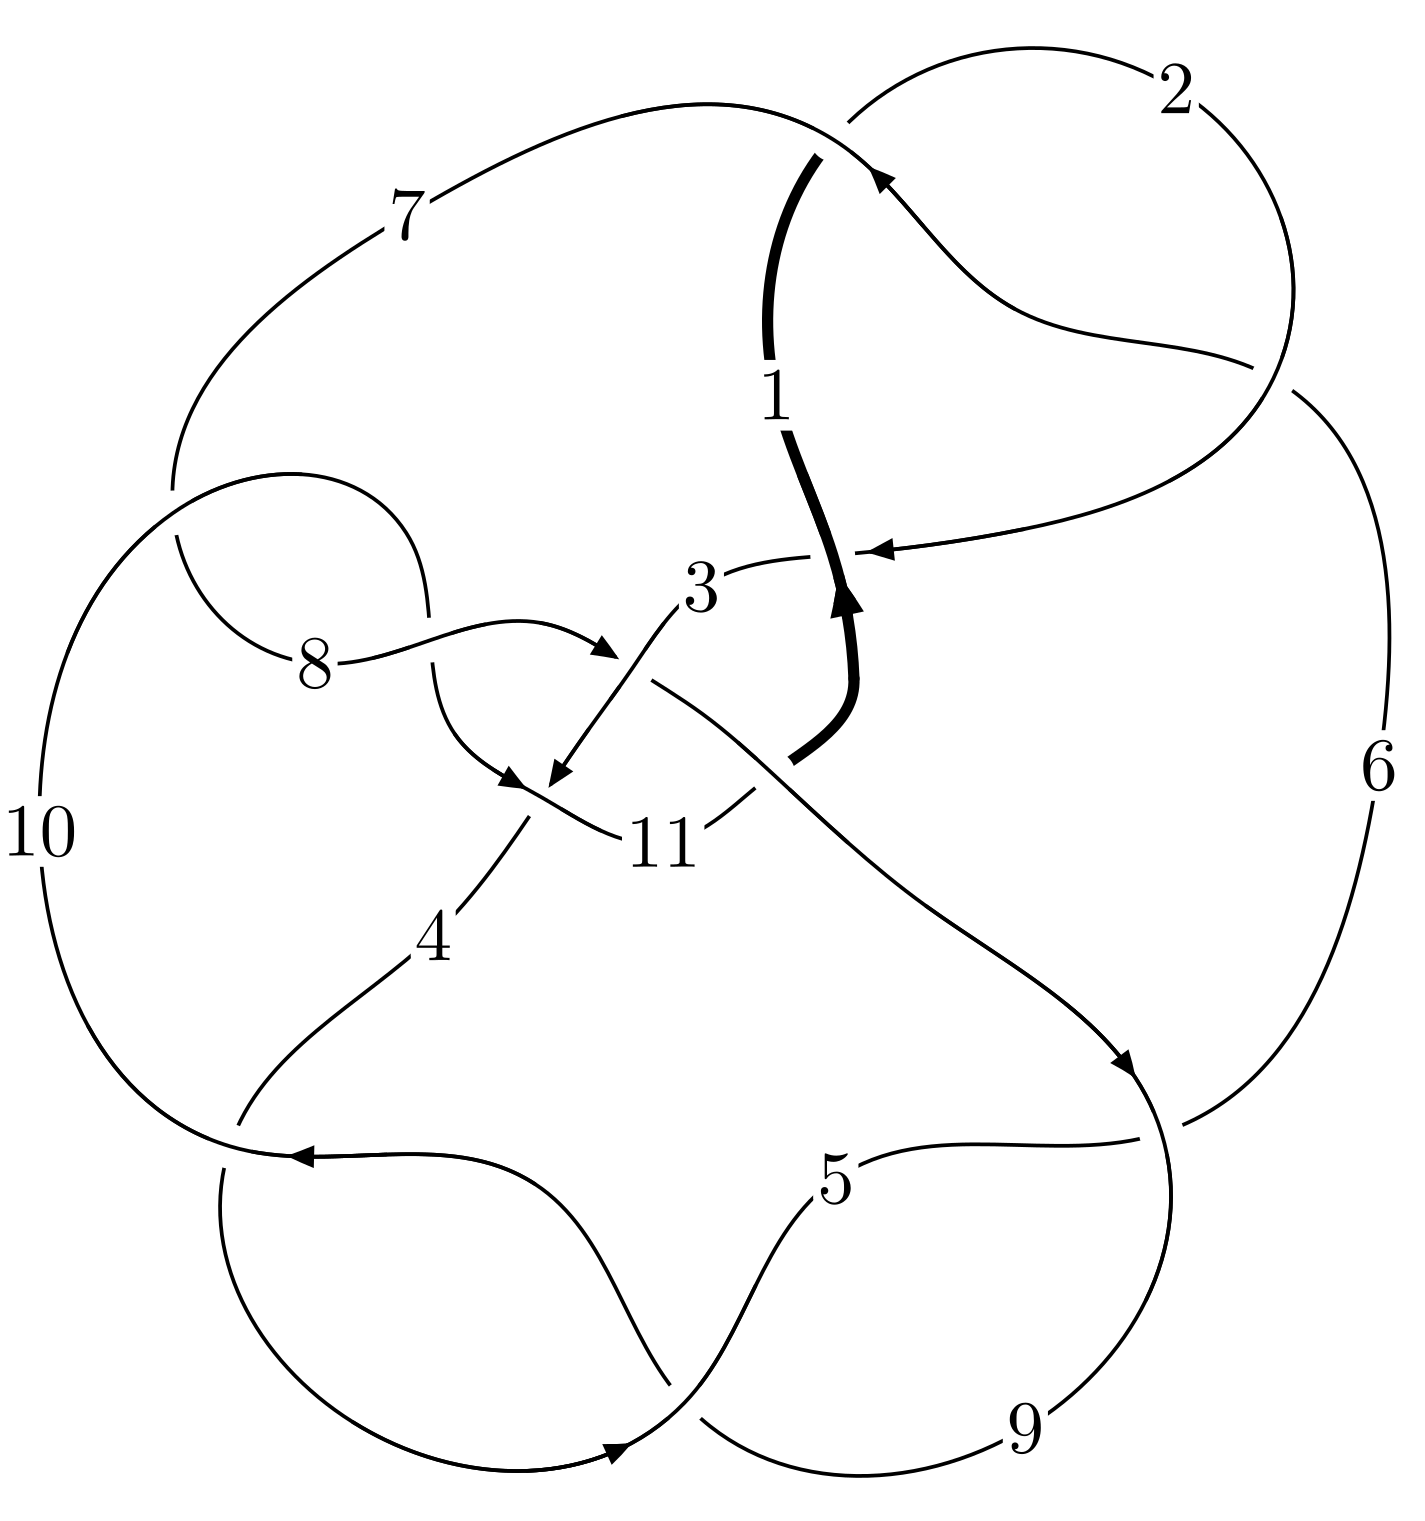
\includegraphics[width=112pt]{../../../GIT/diagram.site/Diagrams/png/731_11n_115.png}\\
\ \ \ A knot diagram\footnotemark}&
\allowdisplaybreaks
\textbf{Linearized knot diagam} \\
\cline{2-2}
 &
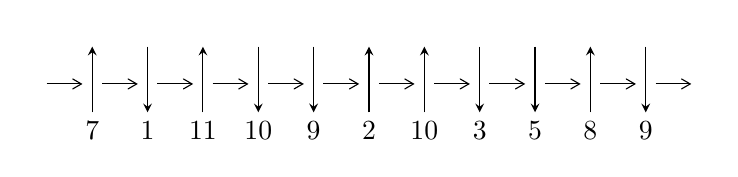
\begin{tikzpicture}[x=20pt, y=17pt]
	% nodes
	\node (C0) at (0, 0) {};
	\node (C1) at (1, 0) {};
	\node (C1U) at (1, +1) {};
	\node (C1D) at (1, -1) {7};

	\node (C2) at (2, 0) {};
	\node (C2U) at (2, +1) {};
	\node (C2D) at (2, -1) {1};

	\node (C3) at (3, 0) {};
	\node (C3U) at (3, +1) {};
	\node (C3D) at (3, -1) {11};

	\node (C4) at (4, 0) {};
	\node (C4U) at (4, +1) {};
	\node (C4D) at (4, -1) {10};

	\node (C5) at (5, 0) {};
	\node (C5U) at (5, +1) {};
	\node (C5D) at (5, -1) {9};

	\node (C6) at (6, 0) {};
	\node (C6U) at (6, +1) {};
	\node (C6D) at (6, -1) {2};

	\node (C7) at (7, 0) {};
	\node (C7U) at (7, +1) {};
	\node (C7D) at (7, -1) {10};

	\node (C8) at (8, 0) {};
	\node (C8U) at (8, +1) {};
	\node (C8D) at (8, -1) {3};

	\node (C9) at (9, 0) {};
	\node (C9U) at (9, +1) {};
	\node (C9D) at (9, -1) {5};

	\node (C10) at (10, 0) {};
	\node (C10U) at (10, +1) {};
	\node (C10D) at (10, -1) {8};

	\node (C11) at (11, 0) {};
	\node (C11U) at (11, +1) {};
	\node (C11D) at (11, -1) {9};
	\node (C12) at (12, 0) {};

	% arrows
	\draw[->,>={angle 60}]
	(C0) edge (C1) (C1) edge (C2) (C2) edge (C3) (C3) edge (C4) (C4) edge (C5) (C5) edge (C6) (C6) edge (C7) (C7) edge (C8) (C8) edge (C9) (C9) edge (C10) (C10) edge (C11) (C11) edge (C12) ;	\draw[->,>=stealth]
	(C1D) edge (C1U) (C2U) edge (C2D) (C3D) edge (C3U) (C4U) edge (C4D) (C5U) edge (C5D) (C6D) edge (C6U) (C7D) edge (C7U) (C8U) edge (C8D) (C9U) edge (C9D) (C10D) edge (C10U) (C11U) edge (C11D) ;
	\end{tikzpicture} \\
\hhline{~~} \\& 
\textbf{Solving Sequence} \\ \cline{2-2} 
 &
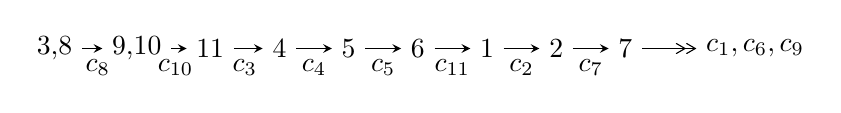
\begin{tikzpicture}[x=25pt, y=7pt]
	% node
	\node (A0) at (-1/8, 0) {3,8};
	\node (A1) at (17/16, 0) {9,10};
	\node (A2) at (17/8, 0) {11};
	\node (A3) at (25/8, 0) {4};
	\node (A4) at (33/8, 0) {5};
	\node (A5) at (41/8, 0) {6};
	\node (A6) at (49/8, 0) {1};
	\node (A7) at (57/8, 0) {2};
	\node (A8) at (65/8, 0) {7};
	\node (C1) at (1/2, -1) {$c_{8}$};
	\node (C2) at (13/8, -1) {$c_{10}$};
	\node (C3) at (21/8, -1) {$c_{3}$};
	\node (C4) at (29/8, -1) {$c_{4}$};
	\node (C5) at (37/8, -1) {$c_{5}$};
	\node (C6) at (45/8, -1) {$c_{11}$};
	\node (C7) at (53/8, -1) {$c_{2}$};
	\node (C8) at (61/8, -1) {$c_{7}$};
	\node (A9) at (10, 0) {$c_{1},c_{6},c_{9}$};

	% edge
	\draw[->,>=stealth]	
	(A0) edge (A1) (A1) edge (A2) (A2) edge (A3) (A3) edge (A4) (A4) edge (A5) (A5) edge (A6) (A6) edge (A7) (A7) edge (A8) ;
	\draw[->>,>={angle 60}]	
	(A8) edge (A9);
\end{tikzpicture} \\ 

\end{tabular} \\

\footnotetext{
The image of knot diagram is generated by the software ``\textbf{Draw programme}" developed by Andrew Bartholomew(\url{http://www.layer8.co.uk/maths/draw/index.htm\#Running-draw}), where we modified some parts for our purpose(\url{https://github.com/CATsTAILs/LinksPainter}).
}\phantom \\ \newline 
\centering \textbf{Ideals for irreducible components\footnotemark of $X_{\text{par}}$} 
 
\begin{align*}
I^u_{1}&=\langle 
-674 u^{17}+4280 u^{16}+\cdots+3857 b+7561,\;5911 u^{17}-7561 u^{16}+\cdots+3857 a-13760,\\
\phantom{I^u_{1}}&\phantom{= \langle  }u^{18}+2 u^{16}+\cdots- u+1\rangle \\
I^u_{2}&=\langle 
-3.99406\times10^{27} u^{29}+7.06888\times10^{27} u^{28}+\cdots+4.03786\times10^{28} b+1.80487\times10^{29},\\
\phantom{I^u_{2}}&\phantom{= \langle  }4.44913\times10^{33} u^{29}-9.50806\times10^{33} u^{28}+\cdots+2.74816\times10^{34} a-2.41871\times10^{35},\;u^{30}- u^{29}+\cdots+4 u+19\rangle \\
I^u_{3}&=\langle 
u^8+4 u^6+u^5+4 u^4+2 u^3+2 u^2+b+2,\;-2 u^8-9 u^6-2 u^5-12 u^4-5 u^3-8 u^2+a-2 u-5,\\
\phantom{I^u_{3}}&\phantom{= \langle  }u^{10}+5 u^8+u^7+8 u^6+3 u^5+6 u^4+2 u^3+4 u^2+1\rangle \\
\\
\end{align*}
\raggedright * 3 irreducible components of $\dim_{\mathbb{C}}=0$, with total 58 representations.\\
\footnotetext{All coefficients of polynomials are rational numbers. But the coefficients are sometimes approximated in decimal forms when there is not enough margin.}
\newpage
\renewcommand{\arraystretch}{1}
\centering \section*{I. $I^u_{1}= \langle -674 u^{17}+4280 u^{16}+\cdots+3857 b+7561,\;5911 u^{17}-7561 u^{16}+\cdots+3857 a-13760,\;u^{18}+2 u^{16}+\cdots- u+1 \rangle$}
\flushleft \textbf{(i) Arc colorings}\\
\begin{tabular}{m{7pt} m{180pt} m{7pt} m{180pt} }
\flushright $a_{3}=$&$\begin{pmatrix}0\\u\end{pmatrix}$ \\
\flushright $a_{8}=$&$\begin{pmatrix}1\\0\end{pmatrix}$ \\
\flushright $a_{9}=$&$\begin{pmatrix}1\\u^2\end{pmatrix}$ \\
\flushright $a_{10}=$&$\begin{pmatrix}-1.53254 u^{17}+1.96033 u^{16}+\cdots-7.35364 u+3.56754\\0.174747 u^{17}-1.10967 u^{16}+\cdots+3.49287 u-1.96033\end{pmatrix}$ \\
\flushright $a_{11}=$&$\begin{pmatrix}-1.35779 u^{17}+0.850661 u^{16}+\cdots-3.86077 u+1.60721\\0.174747 u^{17}-1.10967 u^{16}+\cdots+3.49287 u-1.96033\end{pmatrix}$ \\
\flushright $a_{4}=$&$\begin{pmatrix}-0.607208 u^{17}-1.35779 u^{16}+\cdots+4.77107 u-3.25356\\0.850661 u^{17}+0.363754 u^{16}+\cdots+0.249417 u+1.35779\end{pmatrix}$ \\
\flushright $a_{5}=$&$\begin{pmatrix}-2.56754 u^{17}-1.53254 u^{16}+\cdots+2.73606 u-4.78610\\1.96033 u^{17}+0.174747 u^{16}+\cdots+2.03500 u+1.53254\end{pmatrix}$ \\
\flushright $a_{6}=$&$\begin{pmatrix}-2.56754 u^{17}-1.53254 u^{16}+\cdots+1.73606 u-4.78610\\1.96033 u^{17}+0.174747 u^{16}+\cdots+2.03500 u+1.53254\end{pmatrix}$ \\
\flushright $a_{1}=$&$\begin{pmatrix}-1.16878 u^{17}+1.31216 u^{16}+\cdots-5.14519 u+2.71688\\-0.0674099 u^{17}-1.24553 u^{16}+\cdots+3.76536 u-2.42183\end{pmatrix}$ \\
\flushright $a_{2}=$&$\begin{pmatrix}0.241379 u^{17}-1.58621 u^{16}+\cdots+6.55172 u-3.72414\\-0.710656 u^{17}+0.607726 u^{16}+\cdots-2.60824 u+2.05678\end{pmatrix}$ \\
\flushright $a_{7}=$&$\begin{pmatrix}-2.19212 u^{17}+0.650246 u^{16}+\cdots-5.41872 u+1.14778\\0.834327 u^{17}+0.200415 u^{16}+\cdots+1.55795 u+0.459424\end{pmatrix}$\\ \flushright $a_{7}=$&$\begin{pmatrix}-2.19212 u^{17}+0.650246 u^{16}+\cdots-5.41872 u+1.14778\\0.834327 u^{17}+0.200415 u^{16}+\cdots+1.55795 u+0.459424\end{pmatrix}$\\&\end{tabular}
\flushleft \textbf{(ii) Obstruction class $= -1$}\\~\\
\flushleft \textbf{(iii) Cusp Shapes $= \frac{54335}{3857} u^{17}+\frac{9431}{3857} u^{16}+\cdots+\frac{110875}{3857} u+\frac{36718}{3857}$}\\~\\
\newpage\renewcommand{\arraystretch}{1}
\flushleft \textbf{(iv) u-Polynomials at the component}\newline \\
\begin{tabular}{m{50pt}|m{274pt}}
Crossings & \hspace{64pt}u-Polynomials at each crossing \\
\hline $$\begin{aligned}c_{1},c_{6}\end{aligned}$$&$\begin{aligned}
&u^{18}+6 u^{17}+\cdots+36 u+8
\end{aligned}$\\
\hline $$\begin{aligned}c_{2}\end{aligned}$$&$\begin{aligned}
&u^{18}+8 u^{17}+\cdots+176 u+64
\end{aligned}$\\
\hline $$\begin{aligned}c_{3}\end{aligned}$$&$\begin{aligned}
&u^{18}+2 u^{17}+\cdots+u+1
\end{aligned}$\\
\hline $$\begin{aligned}c_{4},c_{5},c_{8}\\c_{9}\end{aligned}$$&$\begin{aligned}
&u^{18}+2 u^{16}+\cdots+u+1
\end{aligned}$\\
\hline $$\begin{aligned}c_{7},c_{10}\end{aligned}$$&$\begin{aligned}
&u^{18}+9 u^{17}+\cdots+144 u+32
\end{aligned}$\\
\hline $$\begin{aligned}c_{11}\end{aligned}$$&$\begin{aligned}
&u^{18}-2 u^{17}+\cdots+3 u+1
\end{aligned}$\\
\hline
\end{tabular}\\~\\
\newpage\renewcommand{\arraystretch}{1}
\flushleft \textbf{(v) Riley Polynomials at the component}\newline \\
\begin{tabular}{m{50pt}|m{274pt}}
Crossings & \hspace{64pt}Riley Polynomials at each crossing \\
\hline $$\begin{aligned}c_{1},c_{6}\end{aligned}$$&$\begin{aligned}
&y^{18}+8 y^{17}+\cdots+176 y+64
\end{aligned}$\\
\hline $$\begin{aligned}c_{2}\end{aligned}$$&$\begin{aligned}
&y^{18}+4 y^{17}+\cdots+15104 y+4096
\end{aligned}$\\
\hline $$\begin{aligned}c_{3}\end{aligned}$$&$\begin{aligned}
&y^{18}+16 y^{17}+\cdots+45 y+1
\end{aligned}$\\
\hline $$\begin{aligned}c_{4},c_{5},c_{8}\\c_{9}\end{aligned}$$&$\begin{aligned}
&y^{18}+4 y^{17}+\cdots+11 y+1
\end{aligned}$\\
\hline $$\begin{aligned}c_{7},c_{10}\end{aligned}$$&$\begin{aligned}
&y^{18}-9 y^{17}+\cdots+3328 y+1024
\end{aligned}$\\
\hline $$\begin{aligned}c_{11}\end{aligned}$$&$\begin{aligned}
&y^{18}-18 y^{17}+\cdots+23 y+1
\end{aligned}$\\
\hline
\end{tabular}\\~\\
\newpage\flushleft \textbf{(vi) Complex Volumes and Cusp Shapes}
$$\begin{array}{c|c|c}  
\text{Solutions to }I^u_{1}& \I (\text{vol} + \sqrt{-1}CS) & \text{Cusp shape}\\
 \hline 
\begin{aligned}
u &= \phantom{-}0.727352 + 0.735291 I \\
a &= \phantom{-}0.005136 - 0.376666 I \\
b &= \phantom{-}0.391222 + 1.079500 I\end{aligned}
 & -1.41496 - 2.43414 I & -0.56962 + 3.23695 I \\ \hline\begin{aligned}
u &= \phantom{-}0.727352 - 0.735291 I \\
a &= \phantom{-}0.005136 + 0.376666 I \\
b &= \phantom{-}0.391222 - 1.079500 I\end{aligned}
 & -1.41496 + 2.43414 I & -0.56962 - 3.23695 I \\ \hline\begin{aligned}
u &= -1.000950 + 0.529895 I \\
a &= -0.163201 - 0.016901 I \\
b &= \phantom{-}0.585493 - 0.899860 I\end{aligned}
 & -6.19243 - 0.93127 I & -5.63625 + 0.73799 I \\ \hline\begin{aligned}
u &= -1.000950 - 0.529895 I \\
a &= -0.163201 + 0.016901 I \\
b &= \phantom{-}0.585493 + 0.899860 I\end{aligned}
 & -6.19243 + 0.93127 I & -5.63625 - 0.73799 I \\ \hline\begin{aligned}
u &= \phantom{-}0.889387 + 0.824360 I \\
a &= -1.39177 - 0.79525 I \\
b &= \phantom{-}1.122460 - 0.663095 I\end{aligned}
 & -4.47725 - 4.89257 I & -2.95225 + 5.04135 I \\ \hline\begin{aligned}
u &= \phantom{-}0.889387 - 0.824360 I \\
a &= -1.39177 + 0.79525 I \\
b &= \phantom{-}1.122460 + 0.663095 I\end{aligned}
 & -4.47725 + 4.89257 I & -2.95225 - 5.04135 I \\ \hline\begin{aligned}
u &= -0.815454 + 0.912371 I \\
a &= -0.255737 + 0.447363 I \\
b &= \phantom{-}0.541043 - 1.182370 I\end{aligned}
 & -3.92260 + 7.75219 I & -2.08036 - 6.66160 I \\ \hline\begin{aligned}
u &= -0.815454 - 0.912371 I \\
a &= -0.255737 - 0.447363 I \\
b &= \phantom{-}0.541043 + 1.182370 I\end{aligned}
 & -3.92260 - 7.75219 I & -2.08036 + 6.66160 I \\ \hline\begin{aligned}
u &= \phantom{-}0.022331 + 0.744756 I \\
a &= \phantom{-}2.05987 - 0.16817 I \\
b &= -1.69007 + 0.19497 I\end{aligned}
 & \phantom{-}5.20575 - 2.93660 I & \phantom{-}10.23255 + 0.78681 I \\ \hline\begin{aligned}
u &= \phantom{-}0.022331 - 0.744756 I \\
a &= \phantom{-}2.05987 + 0.16817 I \\
b &= -1.69007 - 0.19497 I\end{aligned}
 & \phantom{-}5.20575 + 2.93660 I & \phantom{-}10.23255 - 0.78681 I\\
 \hline 
 \end{array}$$\newpage$$\begin{array}{c|c|c}  
\text{Solutions to }I^u_{1}& \I (\text{vol} + \sqrt{-1}CS) & \text{Cusp shape}\\
 \hline 
\begin{aligned}
u &= -0.170147 + 0.689243 I \\
a &= -3.56038 + 0.93433 I \\
b &= \phantom{-}1.361340 + 0.183714 I\end{aligned}
 & \phantom{-}4.99266 + 3.58040 I & \phantom{-}11.7317 - 10.3370 I \\ \hline\begin{aligned}
u &= -0.170147 - 0.689243 I \\
a &= -3.56038 - 0.93433 I \\
b &= \phantom{-}1.361340 - 0.183714 I\end{aligned}
 & \phantom{-}4.99266 - 3.58040 I & \phantom{-}11.7317 + 10.3370 I \\ \hline\begin{aligned}
u &= -0.759355 + 1.116940 I \\
a &= -1.62765 + 0.48098 I \\
b &= \phantom{-}1.23701 + 0.74198 I\end{aligned}
 & \phantom{-}1.13316 + 8.99334 I & \phantom{-}2.75713 - 6.03184 I \\ \hline\begin{aligned}
u &= -0.759355 - 1.116940 I \\
a &= -1.62765 - 0.48098 I \\
b &= \phantom{-}1.23701 - 0.74198 I\end{aligned}
 & \phantom{-}1.13316 - 8.99334 I & \phantom{-}2.75713 + 6.03184 I \\ \hline\begin{aligned}
u &= \phantom{-}0.248460 + 0.469643 I \\
a &= \phantom{-}0.948209 - 0.220971 I \\
b &= -0.257868 + 0.489761 I\end{aligned}
 & -0.097050 - 1.164640 I & -1.13861 + 6.02305 I \\ \hline\begin{aligned}
u &= \phantom{-}0.248460 - 0.469643 I \\
a &= \phantom{-}0.948209 + 0.220971 I \\
b &= -0.257868 - 0.489761 I\end{aligned}
 & -0.097050 + 1.164640 I & -1.13861 - 6.02305 I \\ \hline\begin{aligned}
u &= \phantom{-}0.85837 + 1.24910 I \\
a &= -1.51448 - 0.36642 I \\
b &= \phantom{-}1.20938 - 0.80152 I\end{aligned}
 & -1.8070 - 14.7634 I & \phantom{-}0.15571 + 8.71478 I \\ \hline\begin{aligned}
u &= \phantom{-}0.85837 - 1.24910 I \\
a &= -1.51448 + 0.36642 I \\
b &= \phantom{-}1.20938 + 0.80152 I\end{aligned}
 & -1.8070 + 14.7634 I & \phantom{-}0.15571 - 8.71478 I\\
 \hline 
 \end{array}$$\newpage\newpage\renewcommand{\arraystretch}{1}
\centering \section*{II. $I^u_{2}= \langle -3.99\times10^{27} u^{29}+7.07\times10^{27} u^{28}+\cdots+4.04\times10^{28} b+1.80\times10^{29},\;4.45\times10^{33} u^{29}-9.51\times10^{33} u^{28}+\cdots+2.75\times10^{34} a-2.42\times10^{35},\;u^{30}- u^{29}+\cdots+4 u+19 \rangle$}
\flushleft \textbf{(i) Arc colorings}\\
\begin{tabular}{m{7pt} m{180pt} m{7pt} m{180pt} }
\flushright $a_{3}=$&$\begin{pmatrix}0\\u\end{pmatrix}$ \\
\flushright $a_{8}=$&$\begin{pmatrix}1\\0\end{pmatrix}$ \\
\flushright $a_{9}=$&$\begin{pmatrix}1\\u^2\end{pmatrix}$ \\
\flushright $a_{10}=$&$\begin{pmatrix}-0.161895 u^{29}+0.345979 u^{28}+\cdots-16.7463 u+8.80118\\0.0989152 u^{29}-0.175065 u^{28}+\cdots+3.29797 u-4.46987\end{pmatrix}$ \\
\flushright $a_{11}=$&$\begin{pmatrix}-0.0629794 u^{29}+0.170914 u^{28}+\cdots-13.4483 u+4.33131\\0.0989152 u^{29}-0.175065 u^{28}+\cdots+3.29797 u-4.46987\end{pmatrix}$ \\
\flushright $a_{4}=$&$\begin{pmatrix}-0.316971 u^{29}+0.590127 u^{28}+\cdots-27.3471 u+10.7433\\0.176327 u^{29}-0.254041 u^{28}+\cdots+8.35983 u-4.03217\end{pmatrix}$ \\
\flushright $a_{5}=$&$\begin{pmatrix}0.00623793 u^{29}+0.145908 u^{28}+\cdots-4.22733 u+10.5731\\-0.0140293 u^{29}-0.0647144 u^{28}+\cdots-3.03553 u-3.76001\end{pmatrix}$ \\
\flushright $a_{6}=$&$\begin{pmatrix}-0.0130929 u^{29}+0.205656 u^{28}+\cdots-1.91890 u+11.4423\\-0.00894659 u^{29}-0.0916273 u^{28}+\cdots-2.82991 u-4.52791\end{pmatrix}$ \\
\flushright $a_{1}=$&$\begin{pmatrix}-0.215063 u^{29}+0.358791 u^{28}+\cdots-15.9814 u+6.75042\\0.193888 u^{29}-0.280534 u^{28}+\cdots+6.04439 u-5.14994\end{pmatrix}$ \\
\flushright $a_{2}=$&$\begin{pmatrix}-0.444660 u^{29}+0.619051 u^{28}+\cdots-23.4202 u+6.77557\\0.135606 u^{29}-0.158420 u^{28}+\cdots+2.39399 u-0.503494\end{pmatrix}$ \\
\flushright $a_{7}=$&$\begin{pmatrix}0.158988 u^{29}-0.0254505 u^{28}+\cdots+7.44679 u+5.85736\\0.0532312 u^{29}-0.0104417 u^{28}+\cdots+7.25020 u+3.35135\end{pmatrix}$\\ \flushright $a_{7}=$&$\begin{pmatrix}0.158988 u^{29}-0.0254505 u^{28}+\cdots+7.44679 u+5.85736\\0.0532312 u^{29}-0.0104417 u^{28}+\cdots+7.25020 u+3.35135\end{pmatrix}$\\&\end{tabular}
\flushleft \textbf{(ii) Obstruction class $= -1$}\\~\\
\flushleft \textbf{(iii) Cusp Shapes $= 0.436420 u^{29}-0.254006 u^{28}+\cdots+22.7490 u+12.5484$}\\~\\
\newpage\renewcommand{\arraystretch}{1}
\flushleft \textbf{(iv) u-Polynomials at the component}\newline \\
\begin{tabular}{m{50pt}|m{274pt}}
Crossings & \hspace{64pt}u-Polynomials at each crossing \\
\hline $$\begin{aligned}c_{1},c_{6}\end{aligned}$$&$\begin{aligned}
&(u^5- u^4+2 u^3- u^2+u-1)^6
\end{aligned}$\\
\hline $$\begin{aligned}c_{2}\end{aligned}$$&$\begin{aligned}
&(u^5+3 u^4+4 u^3+u^2- u-1)^6
\end{aligned}$\\
\hline $$\begin{aligned}c_{3}\end{aligned}$$&$\begin{aligned}
&u^{30}+3 u^{29}+\cdots-138 u+77
\end{aligned}$\\
\hline $$\begin{aligned}c_{4},c_{5},c_{8}\\c_{9}\end{aligned}$$&$\begin{aligned}
&u^{30}+u^{29}+\cdots-4 u+19
\end{aligned}$\\
\hline $$\begin{aligned}c_{7},c_{10}\end{aligned}$$&$\begin{aligned}
&(u^3- u^2+1)^{10}
\end{aligned}$\\
\hline $$\begin{aligned}c_{11}\end{aligned}$$&$\begin{aligned}
&u^{30}-5 u^{29}+\cdots-182 u+347
\end{aligned}$\\
\hline
\end{tabular}\\~\\
\newpage\renewcommand{\arraystretch}{1}
\flushleft \textbf{(v) Riley Polynomials at the component}\newline \\
\begin{tabular}{m{50pt}|m{274pt}}
Crossings & \hspace{64pt}Riley Polynomials at each crossing \\
\hline $$\begin{aligned}c_{1},c_{6}\end{aligned}$$&$\begin{aligned}
&(y^5+3 y^4+4 y^3+y^2- y-1)^6
\end{aligned}$\\
\hline $$\begin{aligned}c_{2}\end{aligned}$$&$\begin{aligned}
&(y^5- y^4+8 y^3-3 y^2+3 y-1)^6
\end{aligned}$\\
\hline $$\begin{aligned}c_{3}\end{aligned}$$&$\begin{aligned}
&y^{30}-5 y^{29}+\cdots+19456 y+5929
\end{aligned}$\\
\hline $$\begin{aligned}c_{4},c_{5},c_{8}\\c_{9}\end{aligned}$$&$\begin{aligned}
&y^{30}+15 y^{29}+\cdots+6520 y+361
\end{aligned}$\\
\hline $$\begin{aligned}c_{7},c_{10}\end{aligned}$$&$\begin{aligned}
&(y^3- y^2+2 y-1)^{10}
\end{aligned}$\\
\hline $$\begin{aligned}c_{11}\end{aligned}$$&$\begin{aligned}
&y^{30}+3 y^{29}+\cdots+526240 y+120409
\end{aligned}$\\
\hline
\end{tabular}\\~\\
\newpage\flushleft \textbf{(vi) Complex Volumes and Cusp Shapes}
$$\begin{array}{c|c|c}  
\text{Solutions to }I^u_{2}& \I (\text{vol} + \sqrt{-1}CS) & \text{Cusp shape}\\
 \hline 
\begin{aligned}
u &= \phantom{-}0.097323 + 0.949937 I \\
a &= \phantom{-}1.212260 + 0.728023 I \\
b &= -0.877439 + 0.744862 I\end{aligned}
 & \phantom{-}1.58157 - 4.35870 I & \phantom{-}1.97513 + 7.41010 I \\ \hline\begin{aligned}
u &= \phantom{-}0.097323 - 0.949937 I \\
a &= \phantom{-}1.212260 - 0.728023 I \\
b &= -0.877439 - 0.744862 I\end{aligned}
 & \phantom{-}1.58157 + 4.35870 I & \phantom{-}1.97513 - 7.41010 I \\ \hline\begin{aligned}
u &= -0.894293 + 0.564111 I \\
a &= \phantom{-}0.362652 - 0.392414 I \\
b &= -0.877439 + 0.744862 I\end{aligned}
 & -0.49041 - 2.82812 I & \phantom{-}1.00910 + 2.97945 I \\ \hline\begin{aligned}
u &= -0.894293 - 0.564111 I \\
a &= \phantom{-}0.362652 + 0.392414 I \\
b &= -0.877439 - 0.744862 I\end{aligned}
 & -0.49041 + 2.82812 I & \phantom{-}1.00910 - 2.97945 I \\ \hline\begin{aligned}
u &= -0.346958 + 0.849386 I \\
a &= -0.65987 + 1.62762 I \\
b &= \phantom{-}0.754878\phantom{ +0.000000I}\end{aligned}
 & \phantom{-}3.64718\phantom{ +0.000000I} & \phantom{-}7.53837 + 0. I\phantom{ +0.000000I} \\ \hline\begin{aligned}
u &= -0.346958 - 0.849386 I \\
a &= -0.65987 - 1.62762 I \\
b &= \phantom{-}0.754878\phantom{ +0.000000I}\end{aligned}
 & \phantom{-}3.64718\phantom{ +0.000000I} & \phantom{-}7.53837 + 0. I\phantom{ +0.000000I} \\ \hline\begin{aligned}
u &= -0.882791 + 0.663108 I \\
a &= \phantom{-}0.444698 - 0.115781 I \\
b &= -0.877439 - 0.744862 I\end{aligned}
 & \phantom{-}1.58157 + 4.35870 I & \phantom{-}1.97513 - 7.41010 I \\ \hline\begin{aligned}
u &= -0.882791 - 0.663108 I \\
a &= \phantom{-}0.444698 + 0.115781 I \\
b &= -0.877439 + 0.744862 I\end{aligned}
 & \phantom{-}1.58157 - 4.35870 I & \phantom{-}1.97513 + 7.41010 I \\ \hline\begin{aligned}
u &= \phantom{-}0.904883 + 0.733963 I \\
a &= \phantom{-}0.085071 - 0.822649 I \\
b &= \phantom{-}0.754878\phantom{ +0.000000I}\end{aligned}
 & \phantom{-}0.17569 - 4.40083 I & \phantom{-}4.27520 + 3.49859 I \\ \hline\begin{aligned}
u &= \phantom{-}0.904883 - 0.733963 I \\
a &= \phantom{-}0.085071 + 0.822649 I \\
b &= \phantom{-}0.754878\phantom{ +0.000000I}\end{aligned}
 & \phantom{-}0.17569 + 4.40083 I & \phantom{-}4.27520 - 3.49859 I\\
 \hline 
 \end{array}$$\newpage$$\begin{array}{c|c|c}  
\text{Solutions to }I^u_{2}& \I (\text{vol} + \sqrt{-1}CS) & \text{Cusp shape}\\
 \hline 
\begin{aligned}
u &= \phantom{-}0.585019 + 1.018790 I \\
a &= \phantom{-}0.740198 + 0.101986 I \\
b &= -0.877439 + 0.744862 I\end{aligned}
 & \phantom{-}1.58157 - 1.29754 I & \phantom{-}1.97513 - 1.45120 I \\ \hline\begin{aligned}
u &= \phantom{-}0.585019 - 1.018790 I \\
a &= \phantom{-}0.740198 - 0.101986 I \\
b &= -0.877439 - 0.744862 I\end{aligned}
 & \phantom{-}1.58157 + 1.29754 I & \phantom{-}1.97513 + 1.45120 I \\ \hline\begin{aligned}
u &= \phantom{-}0.632383 + 1.027640 I \\
a &= \phantom{-}1.49597 + 0.29038 I \\
b &= -0.877439 + 0.744862 I\end{aligned}
 & -0.49041 - 2.82812 I & \phantom{-}1.00910 + 2.97945 I \\ \hline\begin{aligned}
u &= \phantom{-}0.632383 - 1.027640 I \\
a &= \phantom{-}1.49597 - 0.29038 I \\
b &= -0.877439 - 0.744862 I\end{aligned}
 & -0.49041 + 2.82812 I & \phantom{-}1.00910 - 2.97945 I \\ \hline\begin{aligned}
u &= -0.842320 + 0.905421 I \\
a &= \phantom{-}1.63420 - 0.29238 I \\
b &= -0.877439 - 0.744862 I\end{aligned}
 & -3.96189 - 1.57271 I & -2.25407 + 0.51914 I \\ \hline\begin{aligned}
u &= -0.842320 - 0.905421 I \\
a &= \phantom{-}1.63420 + 0.29238 I \\
b &= -0.877439 + 0.744862 I\end{aligned}
 & -3.96189 + 1.57271 I & -2.25407 - 0.51914 I \\ \hline\begin{aligned}
u &= \phantom{-}0.860992 + 0.996268 I \\
a &= \phantom{-}0.509484 + 0.372562 I \\
b &= -0.877439 - 0.744862 I\end{aligned}
 & -3.96189 - 1.57271 I & -2.25407 + 0.51914 I \\ \hline\begin{aligned}
u &= \phantom{-}0.860992 - 0.996268 I \\
a &= \phantom{-}0.509484 - 0.372562 I \\
b &= -0.877439 + 0.744862 I\end{aligned}
 & -3.96189 + 1.57271 I & -2.25407 - 0.51914 I \\ \hline\begin{aligned}
u &= -0.096403 + 0.609074 I \\
a &= -2.26622 - 2.93679 I \\
b &= \phantom{-}0.754878\phantom{ +0.000000I}\end{aligned}
 & \phantom{-}0.17569 + 4.40083 I & \phantom{-}4.27520 - 3.49859 I \\ \hline\begin{aligned}
u &= -0.096403 - 0.609074 I \\
a &= -2.26622 + 2.93679 I \\
b &= \phantom{-}0.754878\phantom{ +0.000000I}\end{aligned}
 & \phantom{-}0.17569 - 4.40083 I & \phantom{-}4.27520 + 3.49859 I\\
 \hline 
 \end{array}$$\newpage$$\begin{array}{c|c|c}  
\text{Solutions to }I^u_{2}& \I (\text{vol} + \sqrt{-1}CS) & \text{Cusp shape}\\
 \hline 
\begin{aligned}
u &= -0.70579 + 1.22794 I \\
a &= \phantom{-}1.52684 - 0.39422 I \\
b &= -0.877439 - 0.744862 I\end{aligned}
 & -3.96189 + 7.22895 I & -2.25407 - 6.47803 I \\ \hline\begin{aligned}
u &= -0.70579 - 1.22794 I \\
a &= \phantom{-}1.52684 + 0.39422 I \\
b &= -0.877439 + 0.744862 I\end{aligned}
 & -3.96189 - 7.22895 I & -2.25407 + 6.47803 I \\ \hline\begin{aligned}
u &= \phantom{-}1.29743 + 0.57947 I \\
a &= \phantom{-}0.408301 + 0.277952 I \\
b &= -0.877439 - 0.744862 I\end{aligned}
 & -3.96189 + 7.22895 I & -2.25407 - 6.47803 I \\ \hline\begin{aligned}
u &= \phantom{-}1.29743 - 0.57947 I \\
a &= \phantom{-}0.408301 - 0.277952 I \\
b &= -0.877439 + 0.744862 I\end{aligned}
 & -3.96189 - 7.22895 I & -2.25407 + 6.47803 I \\ \hline\begin{aligned}
u &= \phantom{-}0.02684 + 1.44366 I \\
a &= -1.83443 + 0.27491 I \\
b &= \phantom{-}0.754878\phantom{ +0.000000I}\end{aligned}
 & \phantom{-}5.71916 - 1.53058 I & \phantom{-}8.50440 + 4.43065 I \\ \hline\begin{aligned}
u &= \phantom{-}0.02684 - 1.44366 I \\
a &= -1.83443 - 0.27491 I \\
b &= \phantom{-}0.754878\phantom{ +0.000000I}\end{aligned}
 & \phantom{-}5.71916 + 1.53058 I & \phantom{-}8.50440 - 4.43065 I \\ \hline\begin{aligned}
u &= \phantom{-}0.067135 + 0.495411 I \\
a &= \phantom{-}1.17711 - 1.53101 I \\
b &= -0.877439 - 0.744862 I\end{aligned}
 & \phantom{-}1.58157 + 1.29754 I & \phantom{-}1.97513 + 1.45120 I \\ \hline\begin{aligned}
u &= \phantom{-}0.067135 - 0.495411 I \\
a &= \phantom{-}1.17711 + 1.53101 I \\
b &= -0.877439 + 0.744862 I\end{aligned}
 & \phantom{-}1.58157 - 1.29754 I & \phantom{-}1.97513 - 1.45120 I \\ \hline\begin{aligned}
u &= -0.20344 + 1.75702 I \\
a &= -0.888896 + 0.183201 I \\
b &= \phantom{-}0.754878\phantom{ +0.000000I}\end{aligned}
 & \phantom{-}5.71916 + 1.53058 I & \phantom{-}8.50440 - 4.43065 I \\ \hline\begin{aligned}
u &= -0.20344 - 1.75702 I \\
a &= -0.888896 - 0.183201 I \\
b &= \phantom{-}0.754878\phantom{ +0.000000I}\end{aligned}
 & \phantom{-}5.71916 - 1.53058 I & \phantom{-}8.50440 + 4.43065 I\\
 \hline 
 \end{array}$$\newpage\newpage\renewcommand{\arraystretch}{1}
\centering \section*{III. $I^u_{3}= \langle u^8+4 u^6+u^5+4 u^4+2 u^3+2 u^2+b+2,\;-2 u^8-9 u^6+\cdots+a-5,\;u^{10}+5 u^8+\cdots+4 u^2+1 \rangle$}
\flushleft \textbf{(i) Arc colorings}\\
\begin{tabular}{m{7pt} m{180pt} m{7pt} m{180pt} }
\flushright $a_{3}=$&$\begin{pmatrix}0\\u\end{pmatrix}$ \\
\flushright $a_{8}=$&$\begin{pmatrix}1\\0\end{pmatrix}$ \\
\flushright $a_{9}=$&$\begin{pmatrix}1\\u^2\end{pmatrix}$ \\
\flushright $a_{10}=$&$\begin{pmatrix}2 u^8+9 u^6+2 u^5+12 u^4+5 u^3+8 u^2+2 u+5\\- u^8-4 u^6- u^5-4 u^4-2 u^3-2 u^2-2\end{pmatrix}$ \\
\flushright $a_{11}=$&$\begin{pmatrix}u^8+5 u^6+u^5+8 u^4+3 u^3+6 u^2+2 u+3\\- u^8-4 u^6- u^5-4 u^4-2 u^3-2 u^2-2\end{pmatrix}$ \\
\flushright $a_{4}=$&$\begin{pmatrix}2 u^9+9 u^7+2 u^6+11 u^5+5 u^4+4 u^3+u^2+3 u-2\\- u^9-5 u^7- u^6-8 u^5-3 u^4-6 u^3-2 u^2-3 u\end{pmatrix}$ \\
\flushright $a_{5}=$&$\begin{pmatrix}4 u^9+18 u^7+4 u^6+23 u^5+10 u^4+12 u^3+3 u^2+8 u-2\\-2 u^9-9 u^7-2 u^6-12 u^5-5 u^4-8 u^3-2 u^2-5 u\end{pmatrix}$ \\
\flushright $a_{6}=$&$\begin{pmatrix}4 u^9+18 u^7+4 u^6+23 u^5+10 u^4+12 u^3+3 u^2+9 u-2\\-2 u^9-9 u^7-2 u^6-12 u^5-5 u^4-7 u^3-2 u^2-5 u\end{pmatrix}$ \\
\flushright $a_{1}=$&$\begin{pmatrix}2 u^8+9 u^6+2 u^5+12 u^4+5 u^3+7 u^2+2 u+4\\-2 u^8-8 u^6-2 u^5-9 u^4-4 u^3-5 u^2-3\end{pmatrix}$ \\
\flushright $a_{2}=$&$\begin{pmatrix}3 u^9+u^8+14 u^7+7 u^6+20 u^5+12 u^4+13 u^3+4 u^2+9 u-1\\-2 u^9-2 u^8-10 u^7-10 u^6-17 u^5-15 u^4-13 u^3-8 u^2-6 u-2\end{pmatrix}$ \\
\flushright $a_{7}=$&$\begin{pmatrix}u^9-2 u^8+4 u^7-9 u^6+2 u^5-13 u^4-4 u^3-9 u^2- u-6\\- u^9+u^8-4 u^7+4 u^6-3 u^5+5 u^4+u^3+3 u^2- u+3\end{pmatrix}$\\ \flushright $a_{7}=$&$\begin{pmatrix}u^9-2 u^8+4 u^7-9 u^6+2 u^5-13 u^4-4 u^3-9 u^2- u-6\\- u^9+u^8-4 u^7+4 u^6-3 u^5+5 u^4+u^3+3 u^2- u+3\end{pmatrix}$\\&\end{tabular}
\flushleft \textbf{(ii) Obstruction class $= 1$}\\~\\
\flushleft \textbf{(iii) Cusp Shapes $= u^9-5 u^8+3 u^7-17 u^6-6 u^5-13 u^4-13 u^3-5 u^2+u-4$}\\~\\
\newpage\renewcommand{\arraystretch}{1}
\flushleft \textbf{(iv) u-Polynomials at the component}\newline \\
\begin{tabular}{m{50pt}|m{274pt}}
Crossings & \hspace{64pt}u-Polynomials at each crossing \\
\hline $$\begin{aligned}c_{1}\end{aligned}$$&$\begin{aligned}
&u^{10}+u^9+3 u^8+2 u^7+5 u^6+3 u^5+6 u^4+2 u^3+4 u^2+u+1
\end{aligned}$\\
\hline $$\begin{aligned}c_{2}\end{aligned}$$&$\begin{aligned}
&u^{10}+5 u^9+\cdots+7 u+1
\end{aligned}$\\
\hline $$\begin{aligned}c_{3}\end{aligned}$$&$\begin{aligned}
&u^{10}- u^8+3 u^7-3 u^6- u^5+4 u^4-6 u^3+5 u^2-2 u+1
\end{aligned}$\\
\hline $$\begin{aligned}c_{4},c_{5},c_{8}\end{aligned}$$&$\begin{aligned}
&u^{10}+5 u^8+u^7+8 u^6+3 u^5+6 u^4+2 u^3+4 u^2+1
\end{aligned}$\\
\hline $$\begin{aligned}c_{6}\end{aligned}$$&$\begin{aligned}
&u^{10}- u^9+3 u^8-2 u^7+5 u^6-3 u^5+6 u^4-2 u^3+4 u^2- u+1
\end{aligned}$\\
\hline $$\begin{aligned}c_{7}\end{aligned}$$&$\begin{aligned}
&u^{10}+2 u^9-2 u^8-7 u^7-2 u^6+8 u^5+7 u^4-3 u^3-4 u^2+1
\end{aligned}$\\
\hline $$\begin{aligned}c_{9}\end{aligned}$$&$\begin{aligned}
&u^{10}+5 u^8- u^7+8 u^6-3 u^5+6 u^4-2 u^3+4 u^2+1
\end{aligned}$\\
\hline $$\begin{aligned}c_{10}\end{aligned}$$&$\begin{aligned}
&u^{10}-2 u^9-2 u^8+7 u^7-2 u^6-8 u^5+7 u^4+3 u^3-4 u^2+1
\end{aligned}$\\
\hline $$\begin{aligned}c_{11}\end{aligned}$$&$\begin{aligned}
&u^{10}-2 u^9+4 u^8-6 u^7+6 u^6-6 u^5+6 u^4- u^3-2 u^2+1
\end{aligned}$\\
\hline
\end{tabular}\\~\\
\newpage\renewcommand{\arraystretch}{1}
\flushleft \textbf{(v) Riley Polynomials at the component}\newline \\
\begin{tabular}{m{50pt}|m{274pt}}
Crossings & \hspace{64pt}Riley Polynomials at each crossing \\
\hline $$\begin{aligned}c_{1},c_{6}\end{aligned}$$&$\begin{aligned}
&y^{10}+5 y^9+\cdots+7 y+1
\end{aligned}$\\
\hline $$\begin{aligned}c_{2}\end{aligned}$$&$\begin{aligned}
&y^{10}+5 y^9+11 y^8+28 y^7+69 y^6+87 y^5+50 y^4+32 y^3+36 y^2- y+1
\end{aligned}$\\
\hline $$\begin{aligned}c_{3}\end{aligned}$$&$\begin{aligned}
&y^{10}-2 y^9-5 y^8+5 y^7+17 y^6+3 y^5-16 y^4-6 y^3+9 y^2+6 y+1
\end{aligned}$\\
\hline $$\begin{aligned}c_{4},c_{5},c_{8}\\c_{9}\end{aligned}$$&$\begin{aligned}
&y^{10}+10 y^9+\cdots+8 y+1
\end{aligned}$\\
\hline $$\begin{aligned}c_{7},c_{10}\end{aligned}$$&$\begin{aligned}
&y^{10}-8 y^9+\cdots-8 y+1
\end{aligned}$\\
\hline $$\begin{aligned}c_{11}\end{aligned}$$&$\begin{aligned}
&y^{10}+4 y^9+4 y^8+4 y^6+10 y^5+8 y^4-13 y^3+16 y^2-4 y+1
\end{aligned}$\\
\hline
\end{tabular}\\~\\
\newpage\flushleft \textbf{(vi) Complex Volumes and Cusp Shapes}
$$\begin{array}{c|c|c}  
\text{Solutions to }I^u_{3}& \I (\text{vol} + \sqrt{-1}CS) & \text{Cusp shape}\\
 \hline 
\begin{aligned}
u &= \phantom{-}0.417680 + 0.777889 I \\
a &= \phantom{-}0.471406 + 0.198677 I \\
b &= -0.762772 + 0.870583 I\end{aligned}
 & \phantom{-}1.59890 - 2.38428 I & \phantom{-}1.97609 + 6.43885 I \\ \hline\begin{aligned}
u &= \phantom{-}0.417680 - 0.777889 I \\
a &= \phantom{-}0.471406 - 0.198677 I \\
b &= -0.762772 - 0.870583 I\end{aligned}
 & \phantom{-}1.59890 + 2.38428 I & \phantom{-}1.97609 - 6.43885 I \\ \hline\begin{aligned}
u &= -0.666811 + 0.558930 I \\
a &= -0.614575 - 0.894984 I \\
b &= -0.616156 - 0.405644 I\end{aligned}
 & -0.77437 + 5.03997 I & -3.44044 - 8.11191 I \\ \hline\begin{aligned}
u &= -0.666811 - 0.558930 I \\
a &= -0.614575 + 0.894984 I \\
b &= -0.616156 + 0.405644 I\end{aligned}
 & -0.77437 - 5.03997 I & -3.44044 + 8.11191 I \\ \hline\begin{aligned}
u &= \phantom{-}0.041017 + 1.338410 I \\
a &= -1.68567 - 0.13858 I \\
b &= \phantom{-}1.242340 + 0.172736 I\end{aligned}
 & \phantom{-}7.62836 + 2.65528 I & \phantom{-}7.48214 - 3.22986 I \\ \hline\begin{aligned}
u &= \phantom{-}0.041017 - 1.338410 I \\
a &= -1.68567 + 0.13858 I \\
b &= \phantom{-}1.242340 - 0.172736 I\end{aligned}
 & \phantom{-}7.62836 - 2.65528 I & \phantom{-}7.48214 + 3.22986 I \\ \hline\begin{aligned}
u &= \phantom{-}0.102677 + 0.595206 I \\
a &= \phantom{-}3.05538 + 0.64412 I \\
b &= -1.47267 + 0.27428 I\end{aligned}
 & \phantom{-}4.57592 - 3.24415 I & -2.14013 + 2.60549 I \\ \hline\begin{aligned}
u &= \phantom{-}0.102677 - 0.595206 I \\
a &= \phantom{-}3.05538 - 0.64412 I \\
b &= -1.47267 - 0.27428 I\end{aligned}
 & \phantom{-}4.57592 + 3.24415 I & -2.14013 - 2.60549 I \\ \hline\begin{aligned}
u &= \phantom{-}0.10544 + 1.60602 I \\
a &= -1.226540 - 0.081108 I \\
b &= \phantom{-}0.609265 + 0.131578 I\end{aligned}
 & \phantom{-}5.06547 - 1.23703 I & -4.37766 - 1.21888 I \\ \hline\begin{aligned}
u &= \phantom{-}0.10544 - 1.60602 I \\
a &= -1.226540 + 0.081108 I \\
b &= \phantom{-}0.609265 - 0.131578 I\end{aligned}
 & \phantom{-}5.06547 + 1.23703 I & -4.37766 + 1.21888 I\\
 \hline 
 \end{array}$$\newpage
\newpage\renewcommand{\arraystretch}{1}
\centering \section*{ IV. u-Polynomials}
\begin{tabular}{m{50pt}|m{274pt}}
Crossings & \hspace{64pt}u-Polynomials at each crossing \\
\hline $$\begin{aligned}c_{1}\end{aligned}$$&$\begin{aligned}
&(u^5- u^4+2 u^3- u^2+u-1)^6\\
&\cdot(u^{10}+u^9+3 u^8+2 u^7+5 u^6+3 u^5+6 u^4+2 u^3+4 u^2+u+1)\\
&\cdot(u^{18}+6 u^{17}+\cdots+36 u+8)
\end{aligned}$\\
\hline $$\begin{aligned}c_{2}\end{aligned}$$&$\begin{aligned}
&((u^5+3 u^4+4 u^3+u^2- u-1)^6)(u^{10}+5 u^9+\cdots+7 u+1)\\
&\cdot(u^{18}+8 u^{17}+\cdots+176 u+64)
\end{aligned}$\\
\hline $$\begin{aligned}c_{3}\end{aligned}$$&$\begin{aligned}
&(u^{10}- u^8+3 u^7-3 u^6- u^5+4 u^4-6 u^3+5 u^2-2 u+1)\\
&\cdot(u^{18}+2 u^{17}+\cdots+u+1)(u^{30}+3 u^{29}+\cdots-138 u+77)
\end{aligned}$\\
\hline $$\begin{aligned}c_{4},c_{5},c_{8}\end{aligned}$$&$\begin{aligned}
&(u^{10}+5 u^8+u^7+8 u^6+3 u^5+6 u^4+2 u^3+4 u^2+1)\\
&\cdot(u^{18}+2 u^{16}+\cdots+u+1)(u^{30}+u^{29}+\cdots-4 u+19)
\end{aligned}$\\
\hline $$\begin{aligned}c_{6}\end{aligned}$$&$\begin{aligned}
&(u^5- u^4+2 u^3- u^2+u-1)^6\\
&\cdot(u^{10}- u^9+3 u^8-2 u^7+5 u^6-3 u^5+6 u^4-2 u^3+4 u^2- u+1)\\
&\cdot(u^{18}+6 u^{17}+\cdots+36 u+8)
\end{aligned}$\\
\hline $$\begin{aligned}c_{7}\end{aligned}$$&$\begin{aligned}
&((u^3- u^2+1)^{10})(u^{10}+2 u^9+\cdots-4 u^2+1)\\
&\cdot(u^{18}+9 u^{17}+\cdots+144 u+32)
\end{aligned}$\\
\hline $$\begin{aligned}c_{9}\end{aligned}$$&$\begin{aligned}
&(u^{10}+5 u^8- u^7+8 u^6-3 u^5+6 u^4-2 u^3+4 u^2+1)\\
&\cdot(u^{18}+2 u^{16}+\cdots+u+1)(u^{30}+u^{29}+\cdots-4 u+19)
\end{aligned}$\\
\hline $$\begin{aligned}c_{10}\end{aligned}$$&$\begin{aligned}
&((u^3- u^2+1)^{10})(u^{10}-2 u^9+\cdots-4 u^2+1)\\
&\cdot(u^{18}+9 u^{17}+\cdots+144 u+32)
\end{aligned}$\\
\hline $$\begin{aligned}c_{11}\end{aligned}$$&$\begin{aligned}
&(u^{10}-2 u^9+4 u^8-6 u^7+6 u^6-6 u^5+6 u^4- u^3-2 u^2+1)\\
&\cdot(u^{18}-2 u^{17}+\cdots+3 u+1)(u^{30}-5 u^{29}+\cdots-182 u+347)
\end{aligned}$\\
\hline
\end{tabular}\newpage\renewcommand{\arraystretch}{1}
\centering \section*{ V. Riley Polynomials}
\begin{tabular}{m{50pt}|m{274pt}}
Crossings & \hspace{64pt}Riley Polynomials at each crossing \\
\hline $$\begin{aligned}c_{1},c_{6}\end{aligned}$$&$\begin{aligned}
&((y^5+3 y^4+4 y^3+y^2- y-1)^6)(y^{10}+5 y^9+\cdots+7 y+1)\\
&\cdot(y^{18}+8 y^{17}+\cdots+176 y+64)
\end{aligned}$\\
\hline $$\begin{aligned}c_{2}\end{aligned}$$&$\begin{aligned}
&(y^5- y^4+8 y^3-3 y^2+3 y-1)^6\\
&\cdot(y^{10}+5 y^9+11 y^8+28 y^7+69 y^6+87 y^5+50 y^4+32 y^3+36 y^2- y+1)\\
&\cdot(y^{18}+4 y^{17}+\cdots+15104 y+4096)
\end{aligned}$\\
\hline $$\begin{aligned}c_{3}\end{aligned}$$&$\begin{aligned}
&(y^{10}-2 y^9-5 y^8+5 y^7+17 y^6+3 y^5-16 y^4-6 y^3+9 y^2+6 y+1)\\
&\cdot(y^{18}+16 y^{17}+\cdots+45 y+1)(y^{30}-5 y^{29}+\cdots+19456 y+5929)
\end{aligned}$\\
\hline $$\begin{aligned}c_{4},c_{5},c_{8}\\c_{9}\end{aligned}$$&$\begin{aligned}
&(y^{10}+10 y^9+\cdots+8 y+1)(y^{18}+4 y^{17}+\cdots+11 y+1)\\
&\cdot(y^{30}+15 y^{29}+\cdots+6520 y+361)
\end{aligned}$\\
\hline $$\begin{aligned}c_{7},c_{10}\end{aligned}$$&$\begin{aligned}
&((y^3- y^2+2 y-1)^{10})(y^{10}-8 y^9+\cdots-8 y+1)\\
&\cdot(y^{18}-9 y^{17}+\cdots+3328 y+1024)
\end{aligned}$\\
\hline $$\begin{aligned}c_{11}\end{aligned}$$&$\begin{aligned}
&(y^{10}+4 y^9+4 y^8+4 y^6+10 y^5+8 y^4-13 y^3+16 y^2-4 y+1)\\
&\cdot(y^{18}-18 y^{17}+\cdots+23 y+1)(y^{30}+3 y^{29}+\cdots+526240 y+120409)
\end{aligned}$\\
\hline
\end{tabular}
\vskip 2pc
\end{document}